% Options for packages loaded elsewhere
% Options for packages loaded elsewhere
\PassOptionsToPackage{unicode}{hyperref}
\PassOptionsToPackage{hyphens}{url}
\PassOptionsToPackage{dvipsnames,svgnames,x11names}{xcolor}
%
\documentclass[
  letterpaper,
  DIV=11,
  numbers=noendperiod]{scrartcl}
\usepackage{xcolor}
\usepackage{amsmath,amssymb}
\setcounter{secnumdepth}{5}
\usepackage{iftex}
\ifPDFTeX
  \usepackage[T1]{fontenc}
  \usepackage[utf8]{inputenc}
  \usepackage{textcomp} % provide euro and other symbols
\else % if luatex or xetex
  \usepackage{unicode-math} % this also loads fontspec
  \defaultfontfeatures{Scale=MatchLowercase}
  \defaultfontfeatures[\rmfamily]{Ligatures=TeX,Scale=1}
\fi
\usepackage{lmodern}
\ifPDFTeX\else
  % xetex/luatex font selection
\fi
% Use upquote if available, for straight quotes in verbatim environments
\IfFileExists{upquote.sty}{\usepackage{upquote}}{}
\IfFileExists{microtype.sty}{% use microtype if available
  \usepackage[]{microtype}
  \UseMicrotypeSet[protrusion]{basicmath} % disable protrusion for tt fonts
}{}
\makeatletter
\@ifundefined{KOMAClassName}{% if non-KOMA class
  \IfFileExists{parskip.sty}{%
    \usepackage{parskip}
  }{% else
    \setlength{\parindent}{0pt}
    \setlength{\parskip}{6pt plus 2pt minus 1pt}}
}{% if KOMA class
  \KOMAoptions{parskip=half}}
\makeatother
% Make \paragraph and \subparagraph free-standing
\makeatletter
\ifx\paragraph\undefined\else
  \let\oldparagraph\paragraph
  \renewcommand{\paragraph}{
    \@ifstar
      \xxxParagraphStar
      \xxxParagraphNoStar
  }
  \newcommand{\xxxParagraphStar}[1]{\oldparagraph*{#1}\mbox{}}
  \newcommand{\xxxParagraphNoStar}[1]{\oldparagraph{#1}\mbox{}}
\fi
\ifx\subparagraph\undefined\else
  \let\oldsubparagraph\subparagraph
  \renewcommand{\subparagraph}{
    \@ifstar
      \xxxSubParagraphStar
      \xxxSubParagraphNoStar
  }
  \newcommand{\xxxSubParagraphStar}[1]{\oldsubparagraph*{#1}\mbox{}}
  \newcommand{\xxxSubParagraphNoStar}[1]{\oldsubparagraph{#1}\mbox{}}
\fi
\makeatother


\usepackage{longtable,booktabs,array}
\newcounter{none} % for unnumbered tables
\usepackage{calc} % for calculating minipage widths
% Correct order of tables after \paragraph or \subparagraph
\usepackage{etoolbox}
\makeatletter
\patchcmd\longtable{\par}{\if@noskipsec\mbox{}\fi\par}{}{}
\makeatother
% Allow footnotes in longtable head/foot
\IfFileExists{footnotehyper.sty}{\usepackage{footnotehyper}}{\usepackage{footnote}}
\makesavenoteenv{longtable}
\usepackage{graphicx}
\makeatletter
\newsavebox\pandoc@box
\newcommand*\pandocbounded[1]{% scales image to fit in text height/width
  \sbox\pandoc@box{#1}%
  \Gscale@div\@tempa{\textheight}{\dimexpr\ht\pandoc@box+\dp\pandoc@box\relax}%
  \Gscale@div\@tempb{\linewidth}{\wd\pandoc@box}%
  \ifdim\@tempb\p@<\@tempa\p@\let\@tempa\@tempb\fi% select the smaller of both
  \ifdim\@tempa\p@<\p@\scalebox{\@tempa}{\usebox\pandoc@box}%
  \else\usebox{\pandoc@box}%
  \fi%
}
% Set default figure placement to htbp
\def\fps@figure{htbp}
\makeatother


% definitions for citeproc citations
\NewDocumentCommand\citeproctext{}{}
\NewDocumentCommand\citeproc{mm}{%
  \begingroup\def\citeproctext{#2}\cite{#1}\endgroup}
\makeatletter
 % allow citations to break across lines
 \let\@cite@ofmt\@firstofone
 % avoid brackets around text for \cite:
 \def\@biblabel#1{}
 \def\@cite#1#2{{#1\if@tempswa , #2\fi}}
\makeatother
\newlength{\cslhangindent}
\setlength{\cslhangindent}{1.5em}
\newlength{\csllabelwidth}
\setlength{\csllabelwidth}{3em}
\newenvironment{CSLReferences}[2] % #1 hanging-indent, #2 entry-spacing
 {\begin{list}{}{%
  \setlength{\itemindent}{0pt}
  \setlength{\leftmargin}{0pt}
  \setlength{\parsep}{0pt}
  % turn on hanging indent if param 1 is 1
  \ifodd #1
   \setlength{\leftmargin}{\cslhangindent}
   \setlength{\itemindent}{-1\cslhangindent}
  \fi
  % set entry spacing
  \setlength{\itemsep}{#2\baselineskip}}}
 {\end{list}}
\usepackage{calc}
\newcommand{\CSLBlock}[1]{\hfill\break\parbox[t]{\linewidth}{\strut\ignorespaces#1\strut}}
\newcommand{\CSLLeftMargin}[1]{\parbox[t]{\csllabelwidth}{\strut#1\strut}}
\newcommand{\CSLRightInline}[1]{\parbox[t]{\linewidth - \csllabelwidth}{\strut#1\strut}}
\newcommand{\CSLIndent}[1]{\hspace{\cslhangindent}#1}



\setlength{\emergencystretch}{3em} % prevent overfull lines

\providecommand{\tightlist}{%
  \setlength{\itemsep}{0pt}\setlength{\parskip}{0pt}}



 


\KOMAoption{captions}{tableheading}
\makeatletter
\@ifpackageloaded{caption}{}{\usepackage{caption}}
\AtBeginDocument{%
\ifdefined\contentsname
  \renewcommand*\contentsname{Table of contents}
\else
  \newcommand\contentsname{Table of contents}
\fi
\ifdefined\listfigurename
  \renewcommand*\listfigurename{List of Figures}
\else
  \newcommand\listfigurename{List of Figures}
\fi
\ifdefined\listtablename
  \renewcommand*\listtablename{List of Tables}
\else
  \newcommand\listtablename{List of Tables}
\fi
\ifdefined\figurename
  \renewcommand*\figurename{Figure}
\else
  \newcommand\figurename{Figure}
\fi
\ifdefined\tablename
  \renewcommand*\tablename{Table}
\else
  \newcommand\tablename{Table}
\fi
}
\@ifpackageloaded{float}{}{\usepackage{float}}
\floatstyle{ruled}
\@ifundefined{c@chapter}{\newfloat{codelisting}{h}{lop}}{\newfloat{codelisting}{h}{lop}[chapter]}
\floatname{codelisting}{Listing}
\newcommand*\listoflistings{\listof{codelisting}{List of Listings}}
\makeatother
\makeatletter
\makeatother
\makeatletter
\@ifpackageloaded{caption}{}{\usepackage{caption}}
\@ifpackageloaded{subcaption}{}{\usepackage{subcaption}}
\makeatother
\usepackage{bookmark}
\IfFileExists{xurl.sty}{\usepackage{xurl}}{} % add URL line breaks if available
\urlstyle{same}
% fallback for those not using the hyperref driver hyperxmp:
\makeatletter
\@ifundefined{xmpquote}{\newcommand{\xmpquote}[1]{#1}}{}
\makeatother
\hypersetup{
  pdftitle={Connecticut Mirror Data Dashboard},
  pdfauthor={Nicole Choi; Zoe Khan; Bayansulu Tulepbayeva; Ellie Zdancewic},
  pdfkeywords={\xmpquote{Connecticut}, \xmpquote{Census}},
  colorlinks=true,
  linkcolor={blue},
  filecolor={Maroon},
  citecolor={Blue},
  urlcolor={Blue},
  pdfcreator={LaTeX via pandoc}}


\title{Connecticut Mirror Data Dashboard}
\author{Nicole Choi \and Zoe Khan \and Bayansulu Tulepbayeva \and Ellie
Zdancewic}
\date{2026-11-06}
\begin{document}
\maketitle
\begin{abstract}
The American Community Survey (ACS) is the most detailed public source
of demographic and economic data for Connecticut, yet reporters rarely
use it because the Census Bureau's tools are hard to navigate, organize
data by county instead of by town, and offer little historical context.
We build an interactive tool, in partnership with Connecticut (CT)
Mirror, that makes ACS accessible to Connecticut reporters. We restrict
the ACS to Connecticut and its 169 towns, organize roughly 1,200
concepts into 14 reporting beats, flag high-priority variables, and
display historical trends alongside current estimates. Our tool offers a
model for adapting large federal datasets to the needs of a specific
newsroom.
\end{abstract}


\section{Introduction}\label{introduction}

\begin{quote}
The Connecticut (CT) Mirror is a Pulitzer-prize winning non-profit
newspaper based in Hartford, Connecticut(Pazniokas 2026). Through
careful reporting of issues spanning immigration, economics, criminal
justice, and public health, the CT Mirror fills a crucial gap in state
policy reporting in Connecticut. Beat reporters frequently integrate
Connecticut census data in their reporting to provide context on housing
trends, education outcomes, and demographic statistics. However, CT
Mirror reporters lack the technical background to make full use of this
rich dataset. According to CT Mirror reporter Angela Eichhorst,
reporters ``want to be able to look at historical trends and also
compare town by town but they don't know how to use the US 5 year census
data estimates.'' Furthermore some ``reporters don't necessarily know
all of the data that is available to them to look at'' (Angela Eichhorst
2026). Therefore, the goals of the CT Mirror Census Data Dashboard are
twofold: first, to provide a user-friendly simplified tool to engage
with historical and town-by-town census data, and second, to introduce
reporters to the full scope of census data available.
\end{quote}

\subsection{Relevant work}\label{relevant-work}

\begin{quote}
Due to the high-visibility and government sponsorship of the U.S.
Census, there already exist several modes of access to Census data. The
Census Bureau publishes their American Consumer Survey microdata as
interactive and filterable spreadsheets, accessible on their website.
However, effective use of these spreadsheets requires significant
background knowledge on Census variables, and it is not accessible to
the average user. Additionally, while the raw data is accessible from
the interactive spreadsheets, there are no visualizations.
\end{quote}

\begin{figure}

\centering{

\pandocbounded{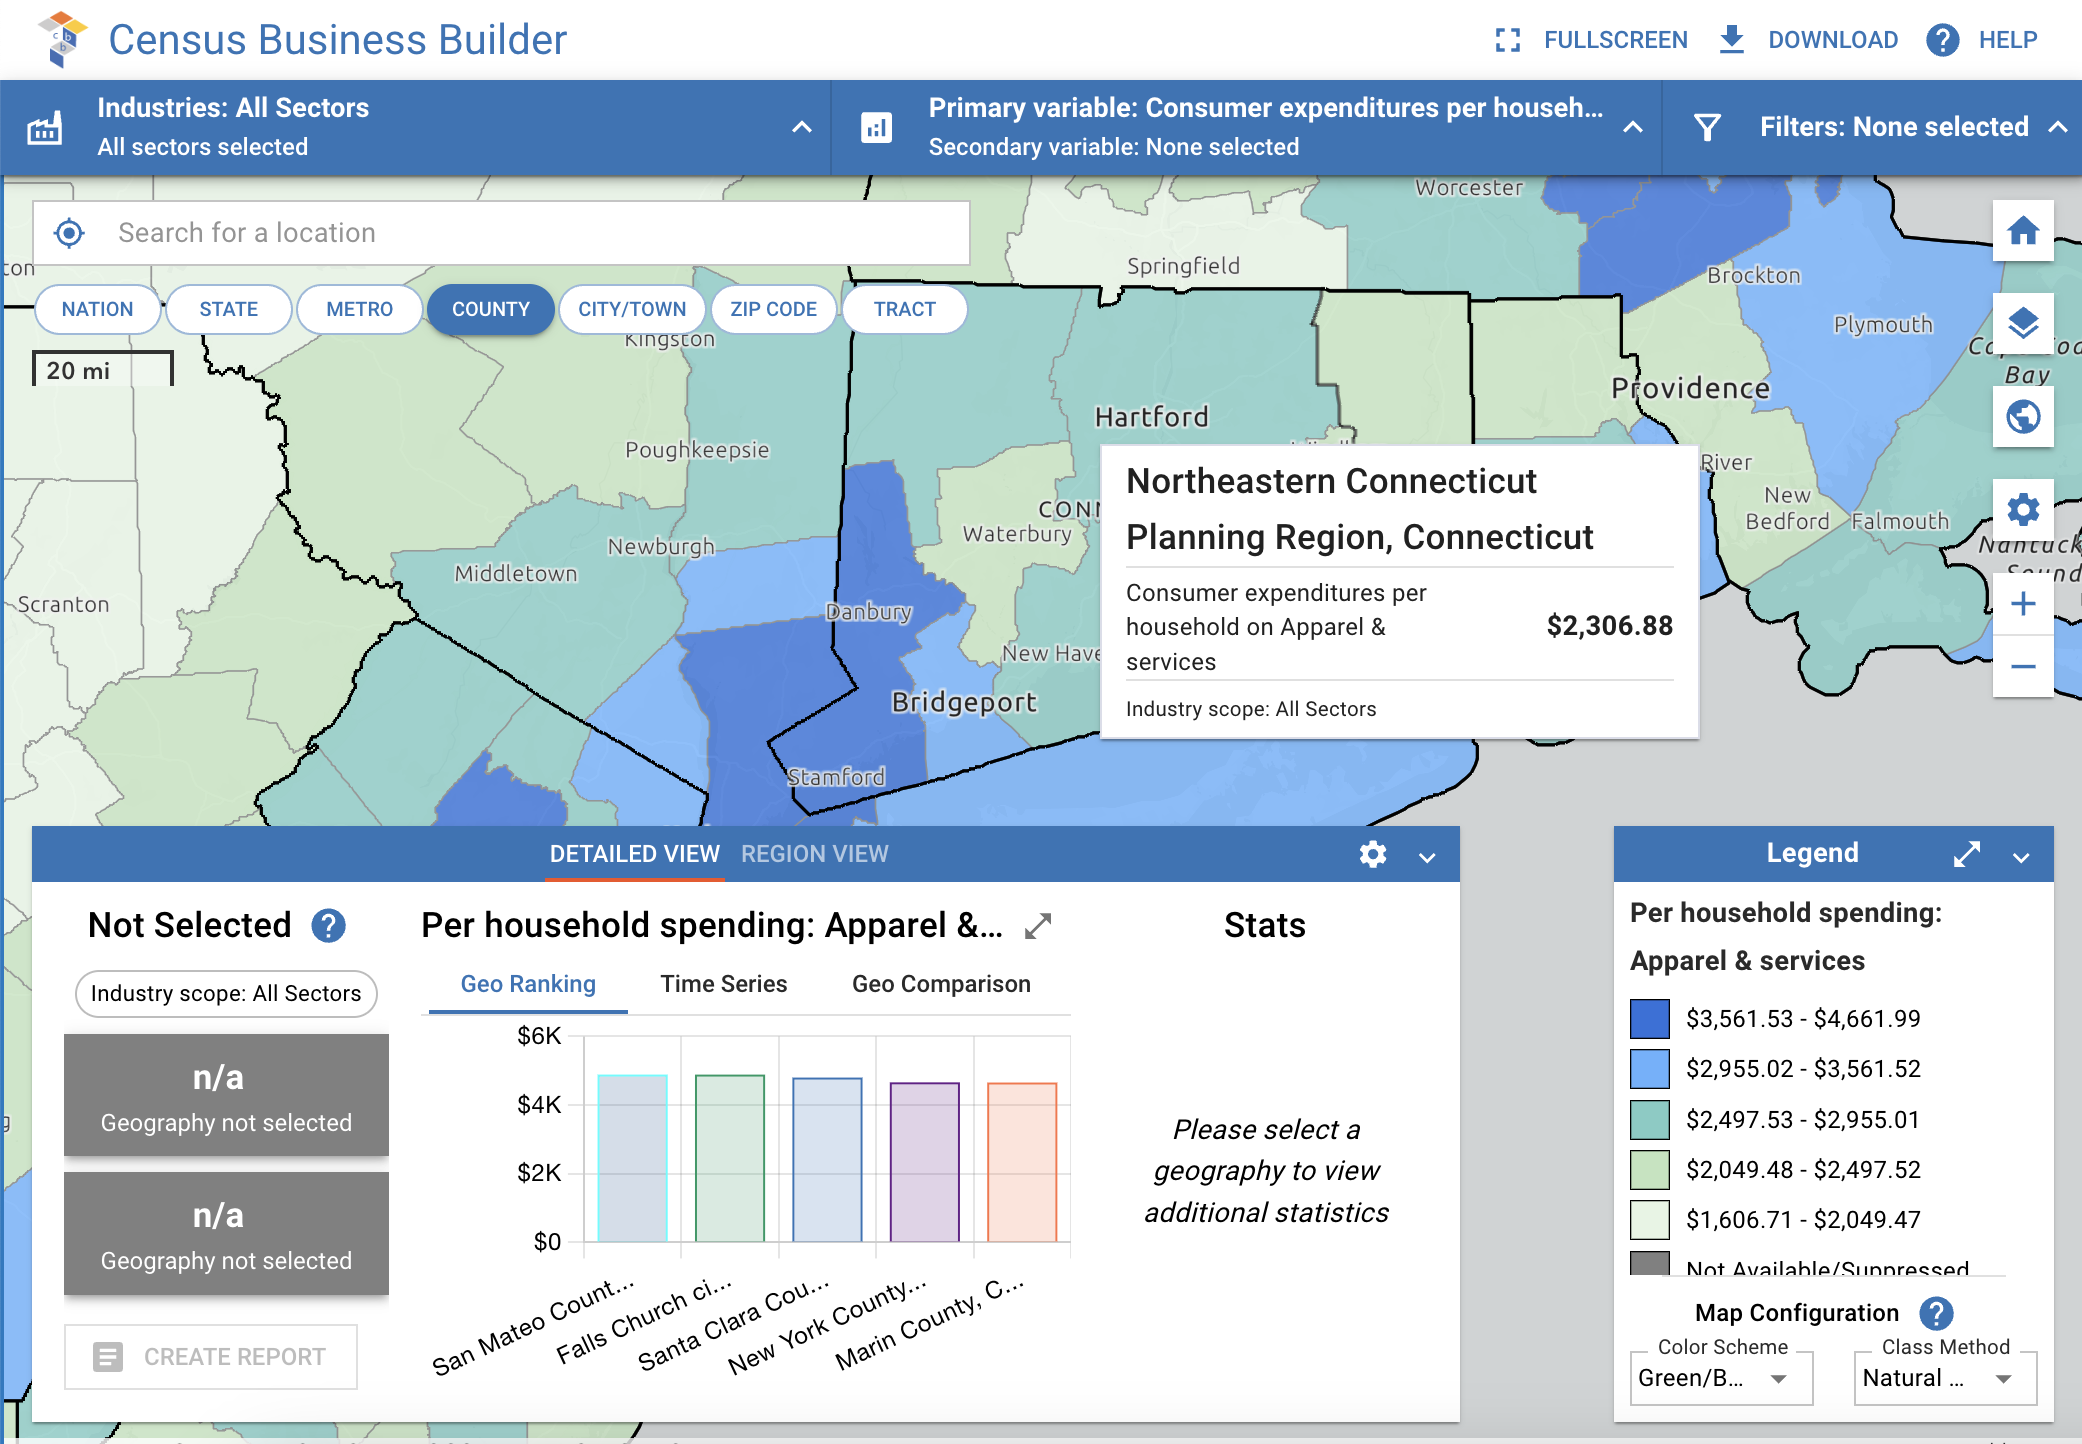
\includegraphics[keepaspectratio]{images/cbb_image.png}}

}

\caption{\label{fig-cbb}Census Business Builder User Interface}

\end{figure}%

\begin{quote}
Alternatively, the Census Bureau publishes a data analytics tool called
the Census Business Builder(US Census Bureau 2026c). This dashboard,
geared towards small business owners, visualizes census data across a
variety of geographies, breaking it down by a primary and secondary
variable as well as a demographic filter. Figure~\ref{fig-cbb} shows a
screenshot of the Census Business Builder User-Interface with one
primary variable selected at the county level. But while the Census
Business Builder is comprehensive, it does not fit the specific needs of
the CTMirror newsroom. The dashboard has a steep learning curve and is
not intuitive for a non-technical user. Additionally, it is not built
for a Connecticut-specific use case. The Census Business Builder has
data on the state, county, and town level. Connecticut, however, doesn't
make legislative decisions on the county-level, making State and Town
the only necessary geographies for this region (Angela Eichhorst 2026).
Finally, the Census Business Builder does not provide historical
time-series data.
\end{quote}

\subsection{Our contribution}\label{our-contribution}

\begin{quote}
This paper presents a new user-friendly, interactive Census Data tool
that is specifically tailored to the needs of reporters in Connecticut.
Unlike existing Census data exploration tools, the Connecticut Mirror
Data Dashboard delivers a time-series analysis of variable trends over
time. Additionally, the final dashboard is streamlined to provide
reporters with the most relevant information as quickly as possible, and
leaving out details that would contribute to user confusion.
\end{quote}

\section{Data}\label{sec-data}

\begin{quote}
The U.S. Census Bureau authors the American Community Survey (ACS), a
publicly available data set used widely by the government (and other
stakeholders) to understand citizens and make data-driven decisions. It
comprises an ongoing survey started in 2005 to collect information about
demographics, education, economics, housing, and more, from sampled
households across the country (US Census Bureau 2026a). About 3.5
million residential addresses are sampled yearly (US Census Bureau
2026b). There are different types of ACS releases, including 1-Year
Estimates, which contains 12-month data for areas with populations of
65,000+ individuals, and 5-Year Estimates, which merges 60-month data
for areas of all population sizes (US Census Bureau 2026b).
\end{quote}

\begin{quote}
All ACS data covers four main categories: Social Characteristics,
Housing Characteristics, Economic Characteristics, Demographic and
Housing Estimates (US Census Bureau 2026a). The ACS organizes its data
as a tree. Concepts form branches and name a broad table topic, such as
Median Household Income in the Past 12 Months. Each concept divides into
subconcepts that break the topic down by categories, such as age group,
race, or sex. The leaves are individual variables, each of which holds
one estimate. The full ACS contains approximately 1,200 concepts and
28,500 subconcepts.
\end{quote}

\begin{figure}

\centering{

\pandocbounded{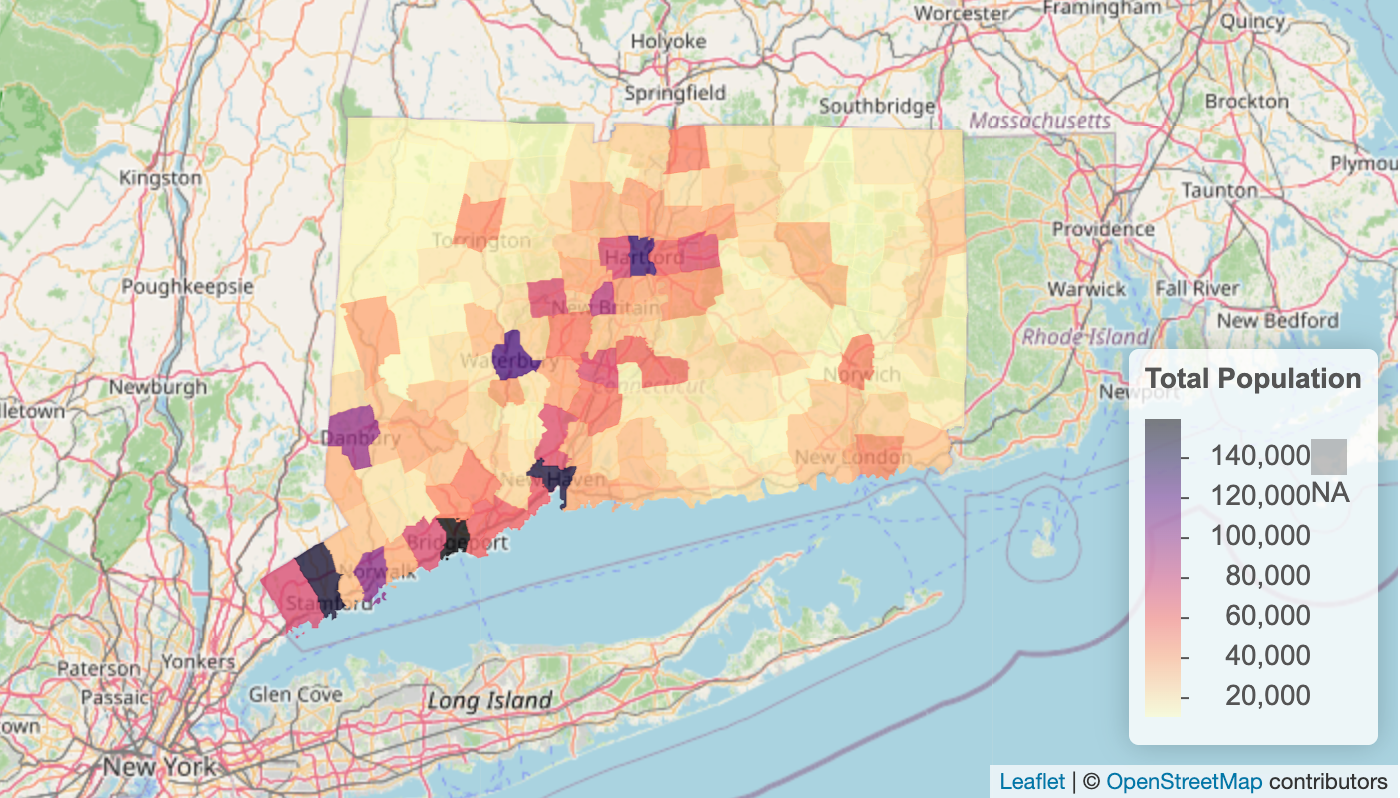
\includegraphics[keepaspectratio]{images/ct_pop_map.png}}

}

\caption{\label{fig-towns}Total Population of Towns in Connecticut in
2024}

\end{figure}%

\begin{quote}
For this project, we restrict our dataset to Connecticut. We keep only
records for the state and its 169 towns. The geographic location and
2024 total population in these towns is displayed in
Figure~\ref{fig-towns}. This restriction removes the national scope that
makes the Census Bureau's own tools hard to navigate and aligns the data
with the geographic units that Connecticut policy uses. The trend of
total population of Connecticut in over the last 19 years is represented
by Figure~\ref{fig-ts}.
\end{quote}

\begin{figure}

\centering{

\pandocbounded{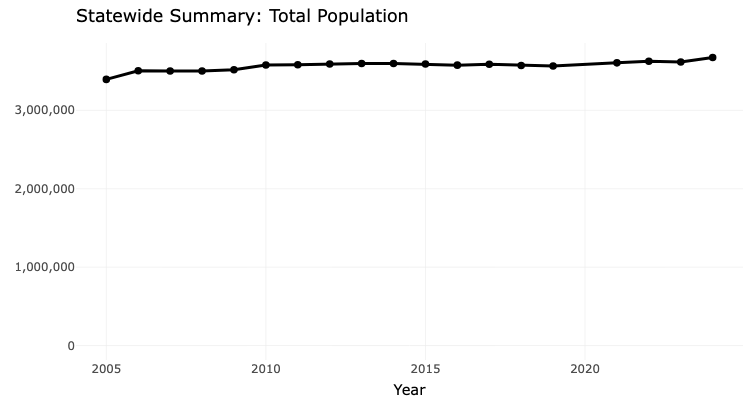
\includegraphics[keepaspectratio]{images/ct_pop_ts.png}}

}

\caption{\label{fig-ts}Connecticut Total Population 2005-2024}

\end{figure}%

\section{Methods}\label{sec-methods}

\begin{quote}
Methods: What did you actually do? What techniques or methods did you
employ? What were the specifications for any statistical models you
used? What software or packages did you use or develop?
\end{quote}

\section{Results}\label{results}

\begin{quote}
Results: What did you learn about the problem you identified in Section
1? This is where you put the tables, figures, and analytics by-products
of your work.
\end{quote}

\section{Conclusion}\label{conclusion}

\begin{quote}
Conclusion: What are the limitations of your work? What are some next
steps that someone (either you or another research group) should
consider in attempting to further your work? Remind us one last time
about what you did.
\end{quote}

\subsection{Limitations}\label{limitations}

\subsection{Future work}\label{future-work}

\subsection{Final thoughts}\label{final-thoughts}

\section{Ethical statement}\label{ethical-statement}

\begin{quote}
Drawing on what you have learned about data science ethics in this
class, discuss any ethical considerations in your project. For some
projects, this statement could be quite short (one paragraph may
suffice). For other projects, more detail may be needed (no more than 2
pages).

Be expansive and creative in your thinking about \textbf{possible}
ethical considerations. One way to do this assignment poorly would be to
write a short statement asserting that there are no ethical
considerations, only to have me think of several fairly obvious ones.
\end{quote}

\section{Acknowledgements}\label{acknowledgements}

\begin{quote}
Were there any people or organizations who helped you that you would
like to acknowledge?
\end{quote}

\section*{References}\label{references}
\addcontentsline{toc}{section}{References}

\begin{quote}
References: Every reference (except for books) needs a DOI (strongly
preferred) or URL. Use \href{https://scholar.google.com}{Google Scholar}
to help with BibTeX. Every book needs publisher location (e.g.~``City,
ST: Publisher''). 🙄 See
\href{https://smithcollege-sds.github.io/sds100/lab_12_bibliographies.html}{SDS
100: Bibliographies}
\end{quote}

\protect\phantomsection\label{refs}
\begin{CSLReferences}{1}{1}
\bibitem[\citeproctext]{ref-angela_eichhorst_connecticut_2026}
Angela Eichhorst. 2026. \emph{Connecticut {Mirror} {Project} {Video}}.

\bibitem[\citeproctext]{ref-pazniokas_ct_2026}
Pazniokas, Mark. 2026. {``{CT} {Mirror} Wins First {Pulitzer} {Prize}
for '{On} the {Hook}' Series.''} In \emph{CT Mirror}.
\url{https://ctmirror.org/2026/05/04/ctmirror-pulitzer-prize-on-the-hook-propublica/}.

\bibitem[\citeproctext]{ref-us_census_bureau_american_2026}
US Census Bureau. 2026a. {``American {Community} {Survey} ({ACS}).''} In
\emph{Census.gov}.
\url{https://www.census.gov/programs-surveys/acs.html}.

\bibitem[\citeproctext]{ref-us_census_bureau_american_2026-1}
US Census Bureau. 2026b. {``American {Community} {Survey} {Information}
{Guide}.''} In \emph{Census.gov}.
\url{https://www.census.gov/programs-surveys/acs/about/information-guide.html}.

\bibitem[\citeproctext]{ref-us_census_bureau_census_2026}
US Census Bureau. 2026c. \emph{Census {Business} {Builder}}.
\url{https://cbb.census.gov/cbb/\#view=map&industries=00&clusterName=Custom+Industries&geoType=state&dataVariable=33&dashboardVars=15-17-1-64&centerX=-10802692&centerY=4568679&level=4&theme=default&dynHeader=Custom+Region}.

\end{CSLReferences}




\end{document}
